L'utilisateur a la possibilité d'afficher le contenu du sac à dos en cliquant sur l'icône sac en bas à droite de l'écran.

\begin{figure}[H]
    \centering
    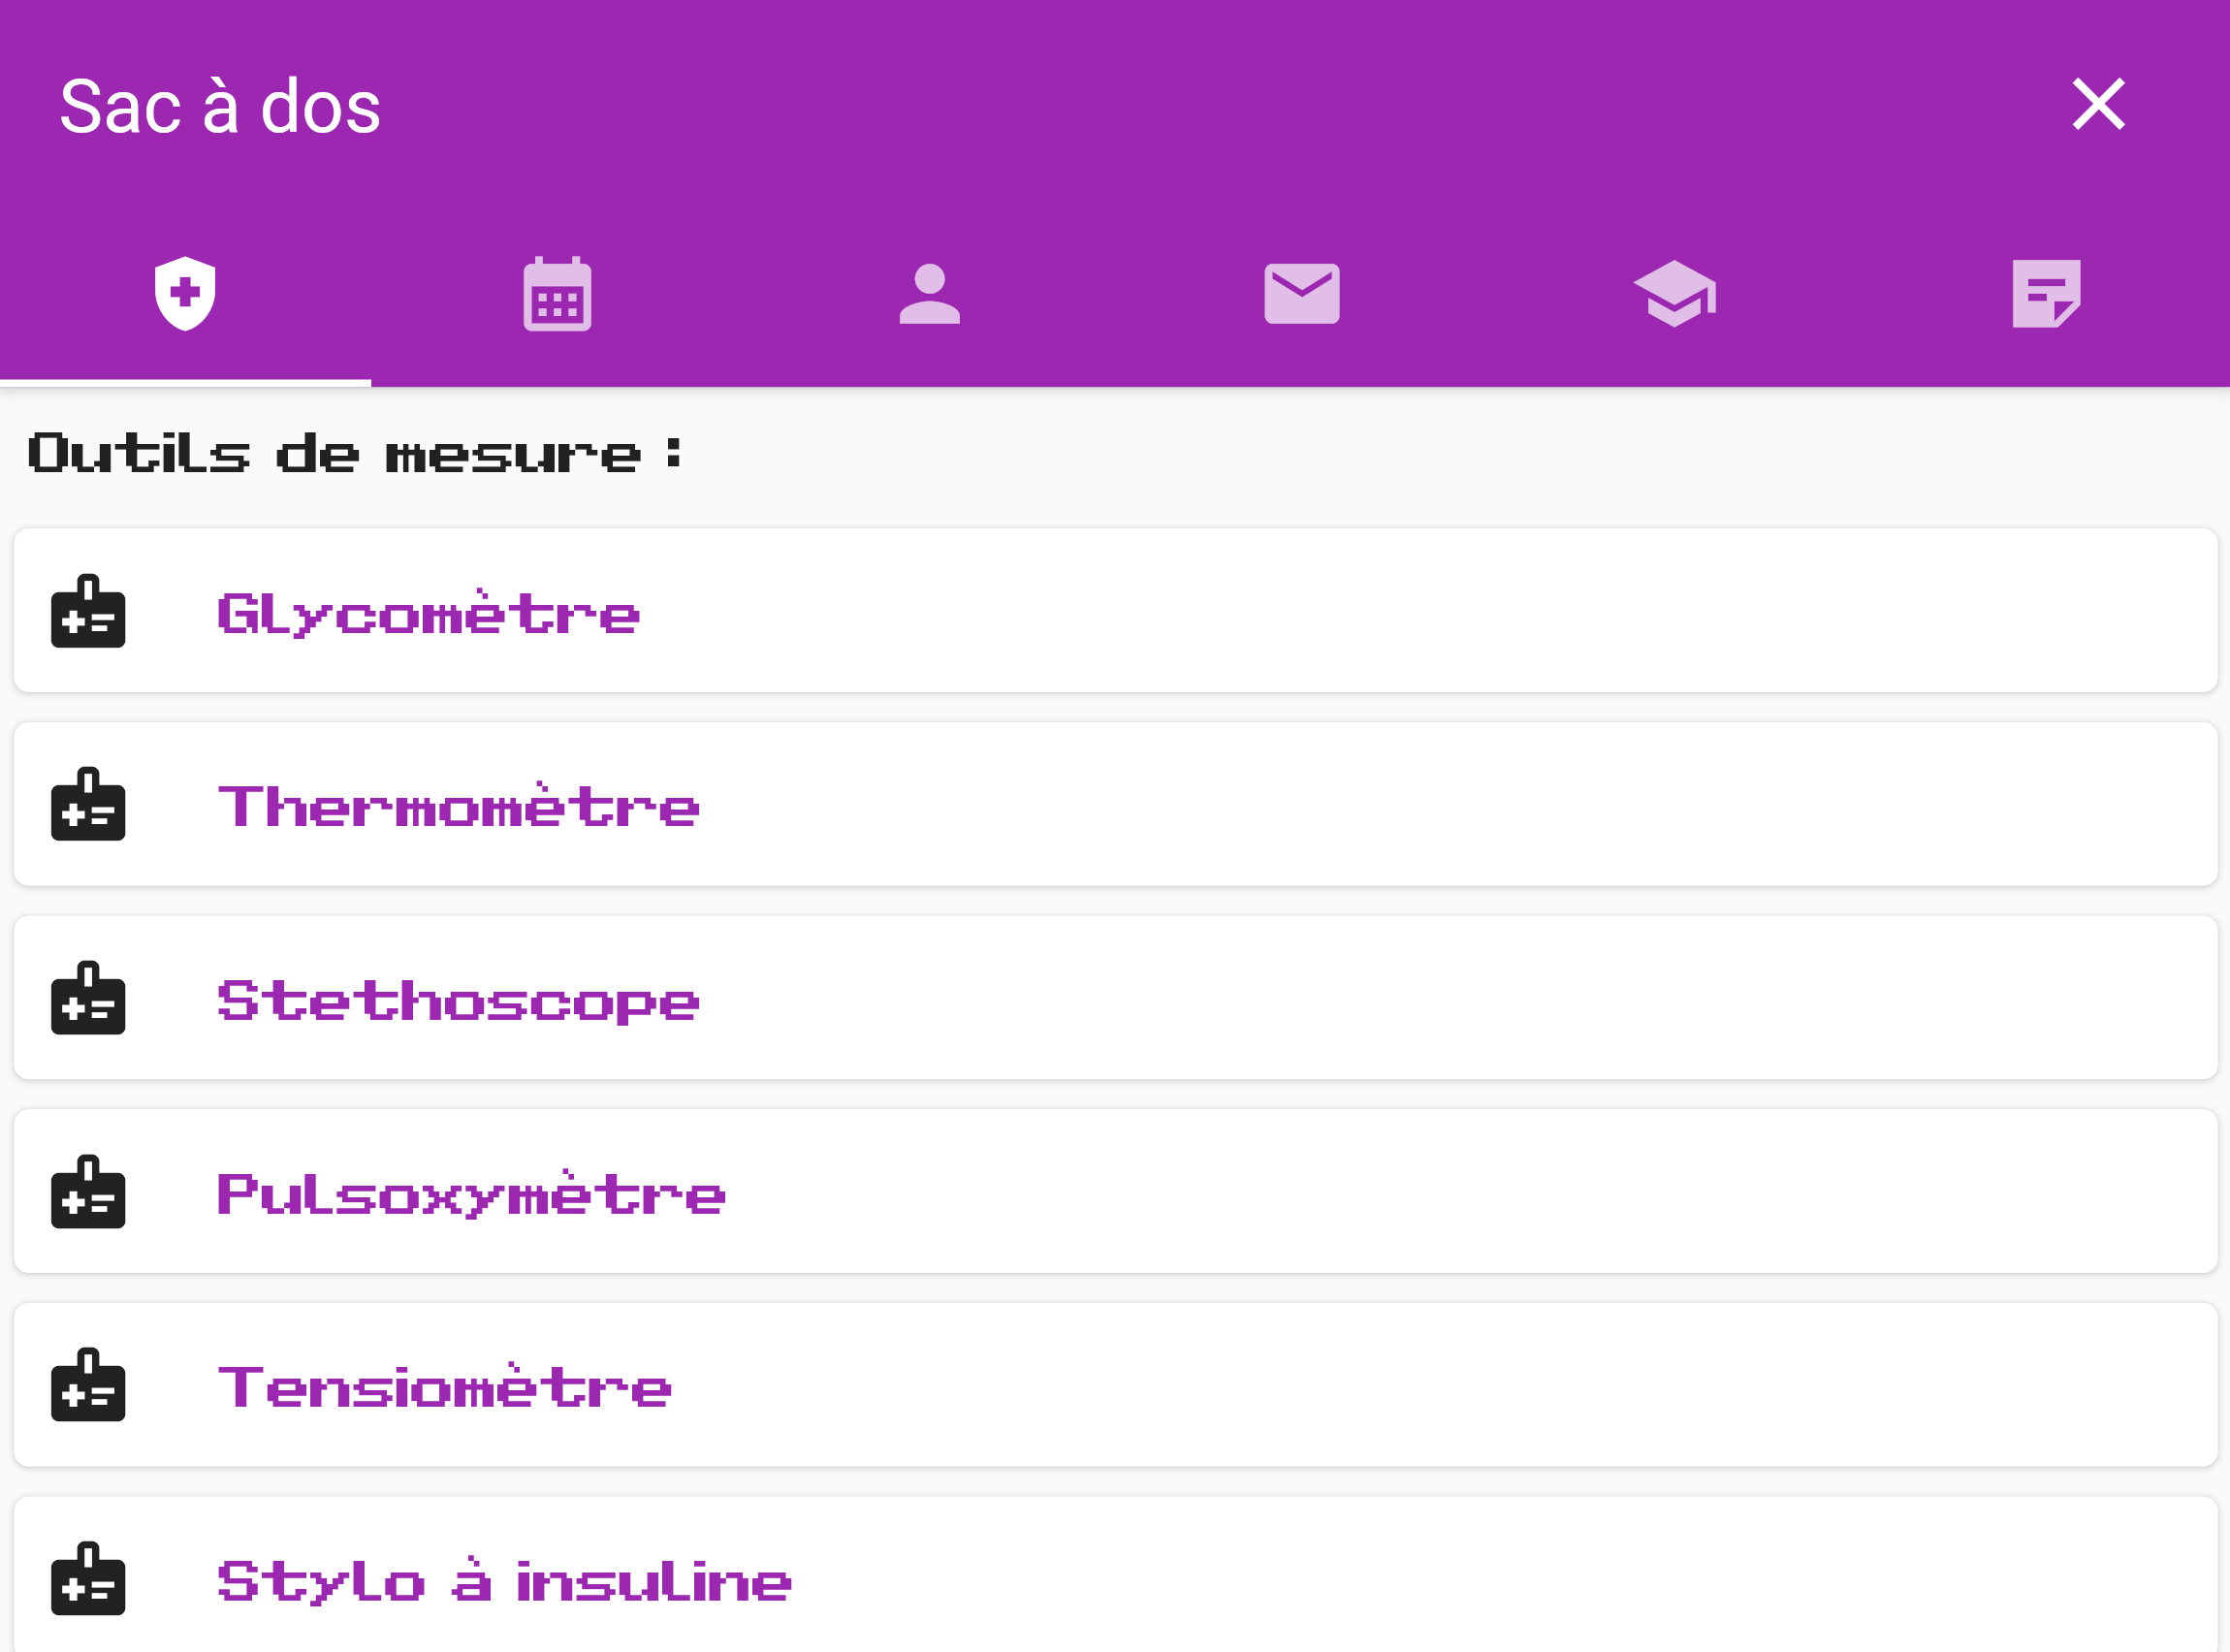
\includegraphics[width=0.8\textwidth ]{images/toolsMenu/toolbox.png}
    \caption{Sac à dos}
    \label{fig:pic_dessus}
\end{figure}

Le sac à dos contient les onglets suivants:
\begin{itemize}
    \item les outils de mesure
    \item le planning de la journée
    \item les situations des patients
    \item la liste de professionnels
    \item la collection des apprentissages
    \item les notes sur les patients
\end{itemize}

%============================================================
%****************Onglet 1 outils*******************

\subsubsection*{Outils de mesure}
\addcontentsline{toc}{subsubsection}{Outils de mesure}

Le premier onglet du menu du sac à dos contient les différents outils de mesure. En cliquant sur cet onglet, l'utilisateur a la possibilité de sélectionner les outils à opérer sur les patients. \\

\begin{figure}[H]
    \centering
    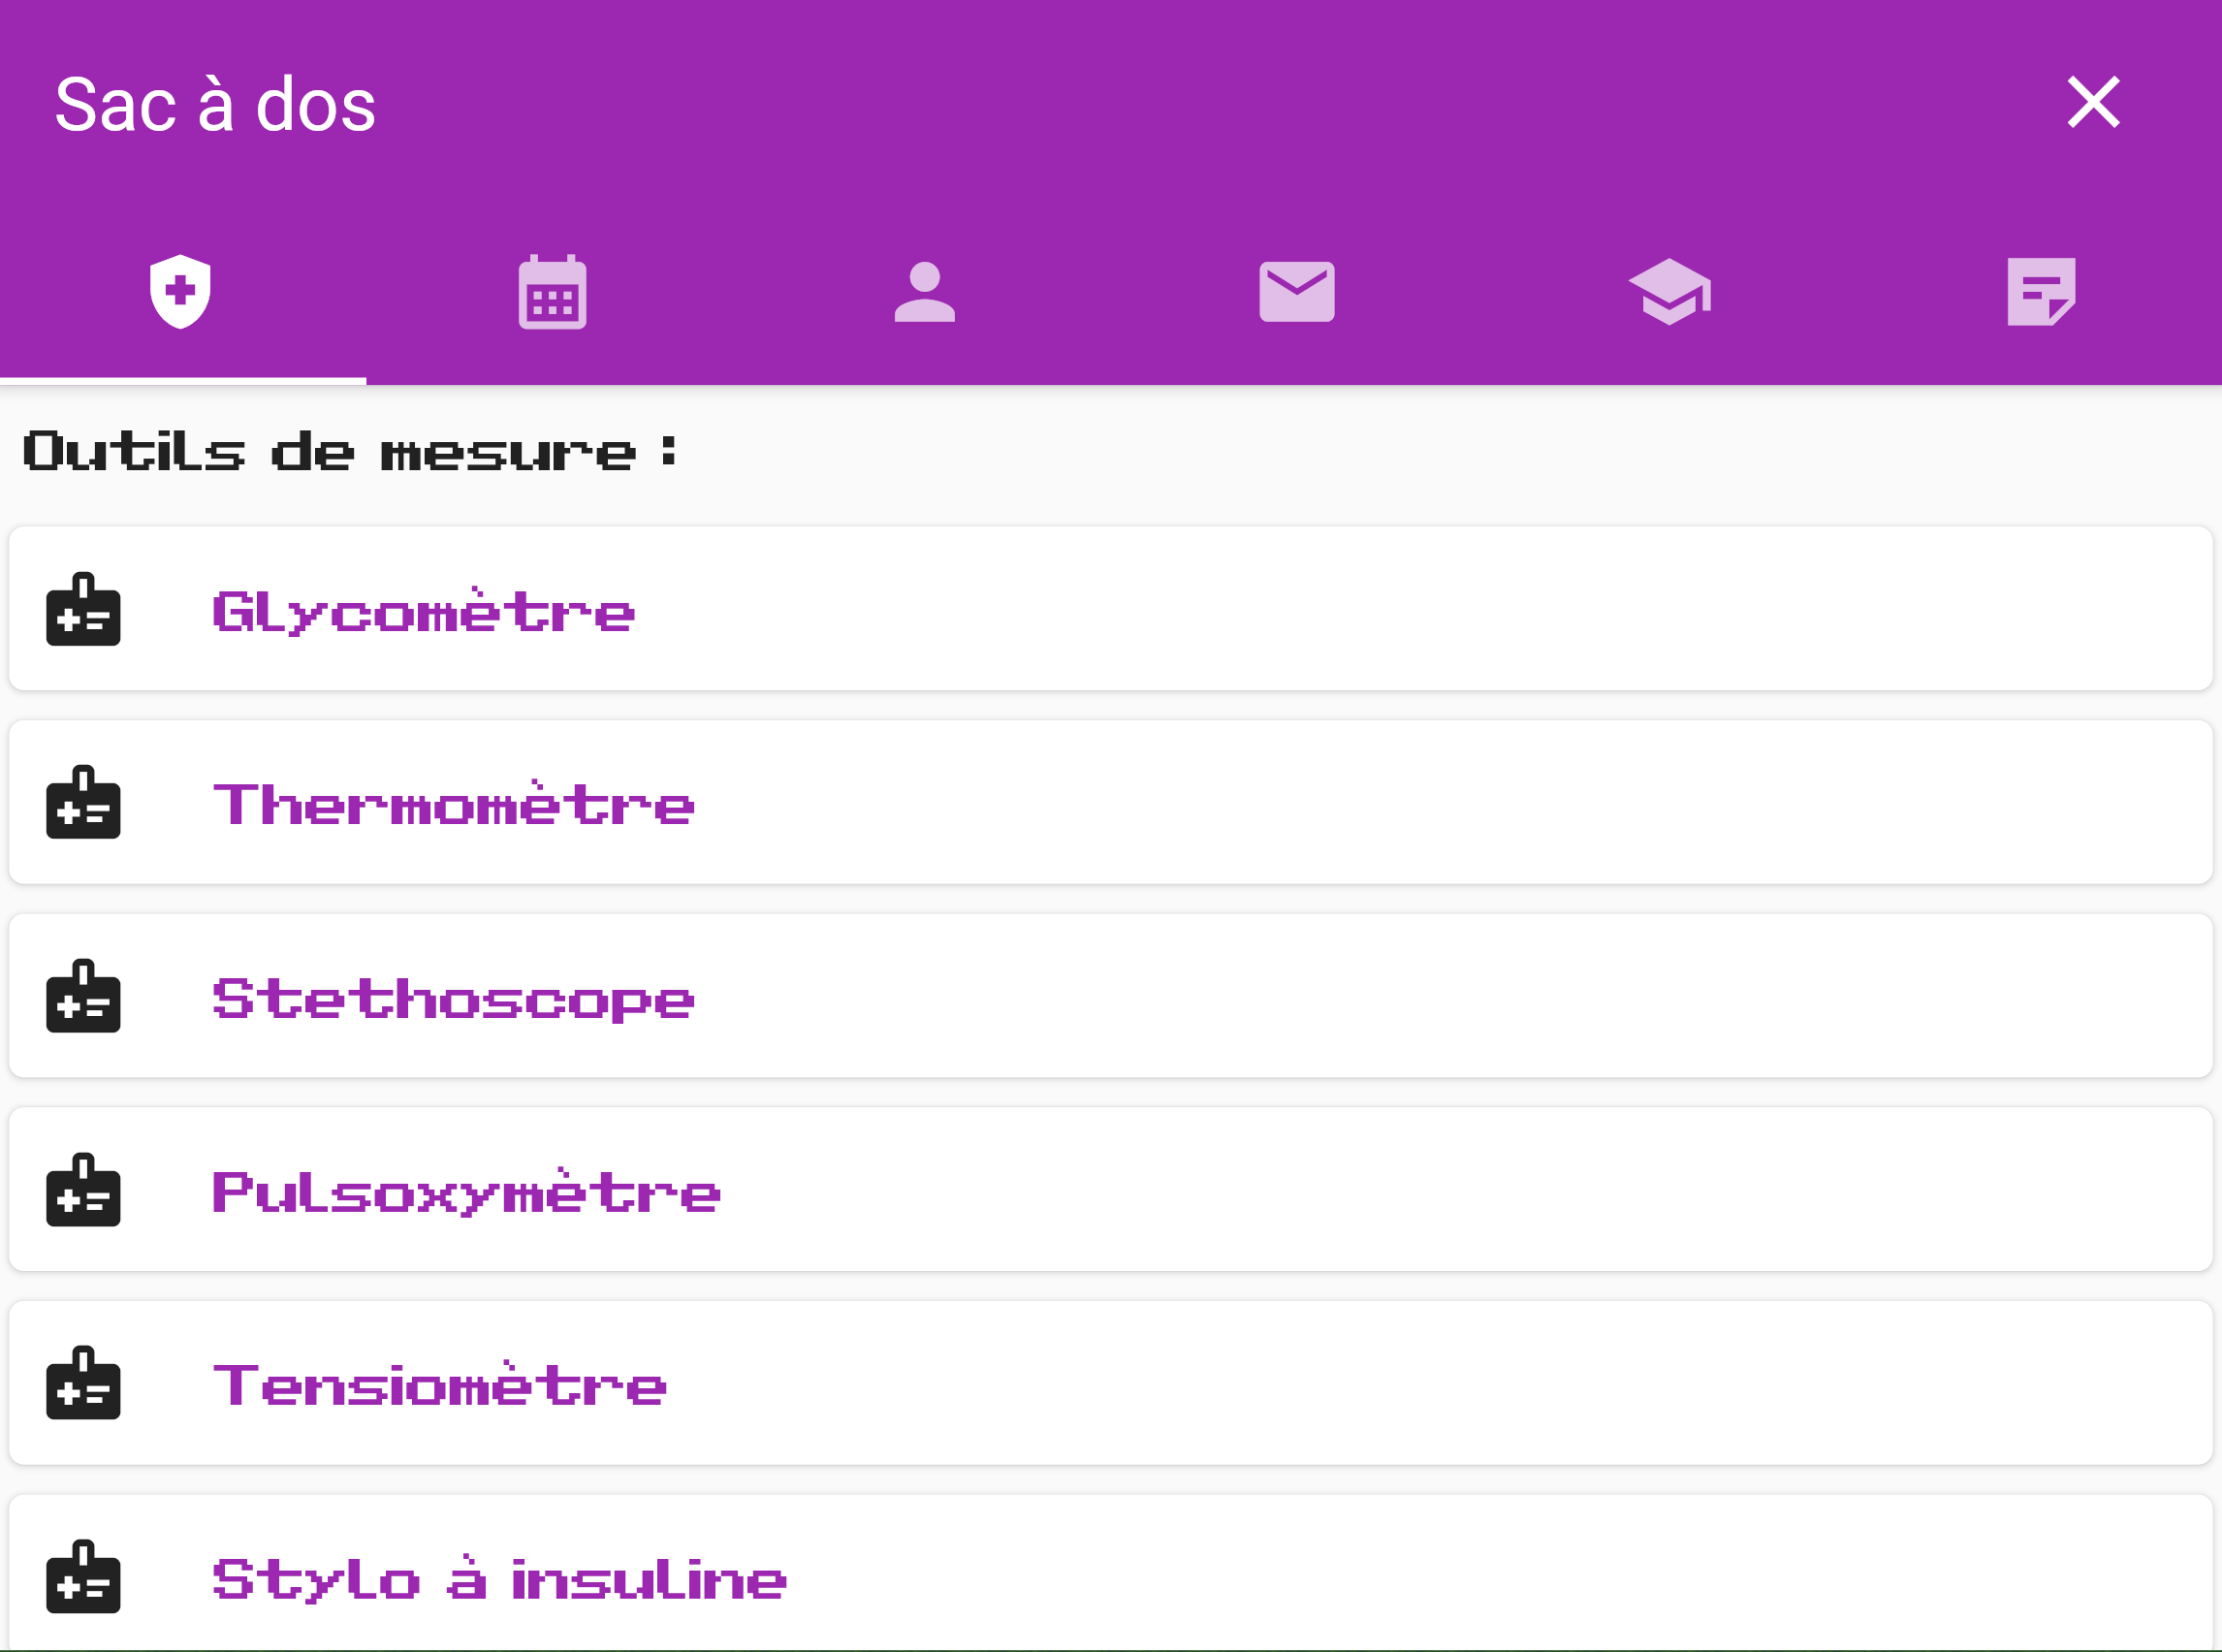
\includegraphics[width=0.8\textwidth ]{images/toolsMenu/tools.png}
    \caption{Sac à dos - Outils de mesure}
    \label{fig:pic_dessus}
\end{figure}

Lorsque nous cliquons sur un outil qui ne peut pas être utilisé, un dialogue nous en avertit.

\begin{figure}[H]
    \centering
    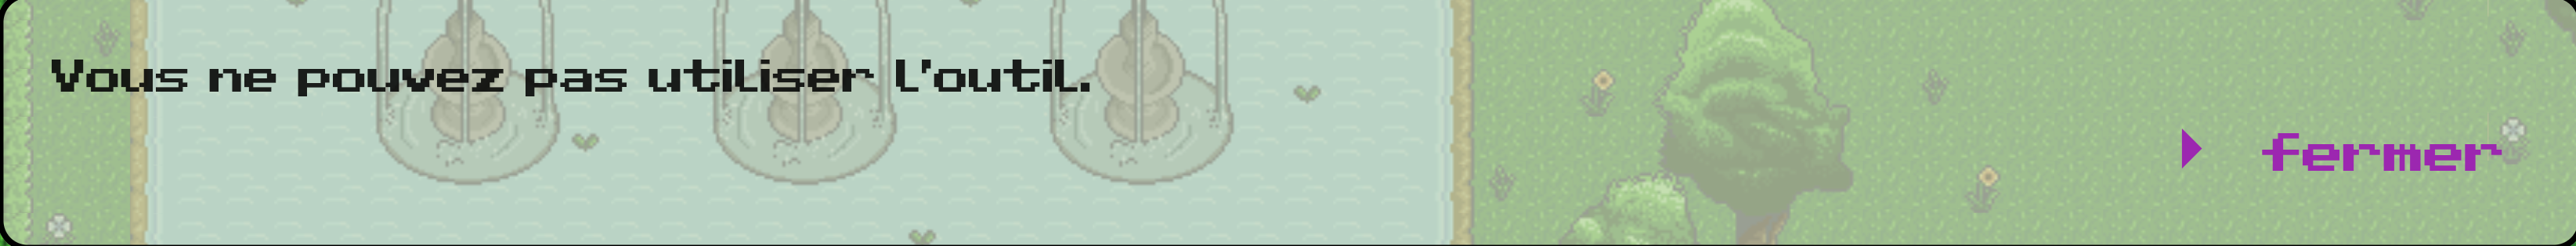
\includegraphics[width=0.8\textwidth ]{images/toolsMenu/toolCantBeUsed.png}
    \caption{Sac à dos - Outils de mesure ne peut être utilisé}
    \label{fig:pic_dessus}
\end{figure}

En revanche, lorsqu'un outil est utilisable, un dialogue indique la mesure prise.
\begin{figure}[H]
    \centering
    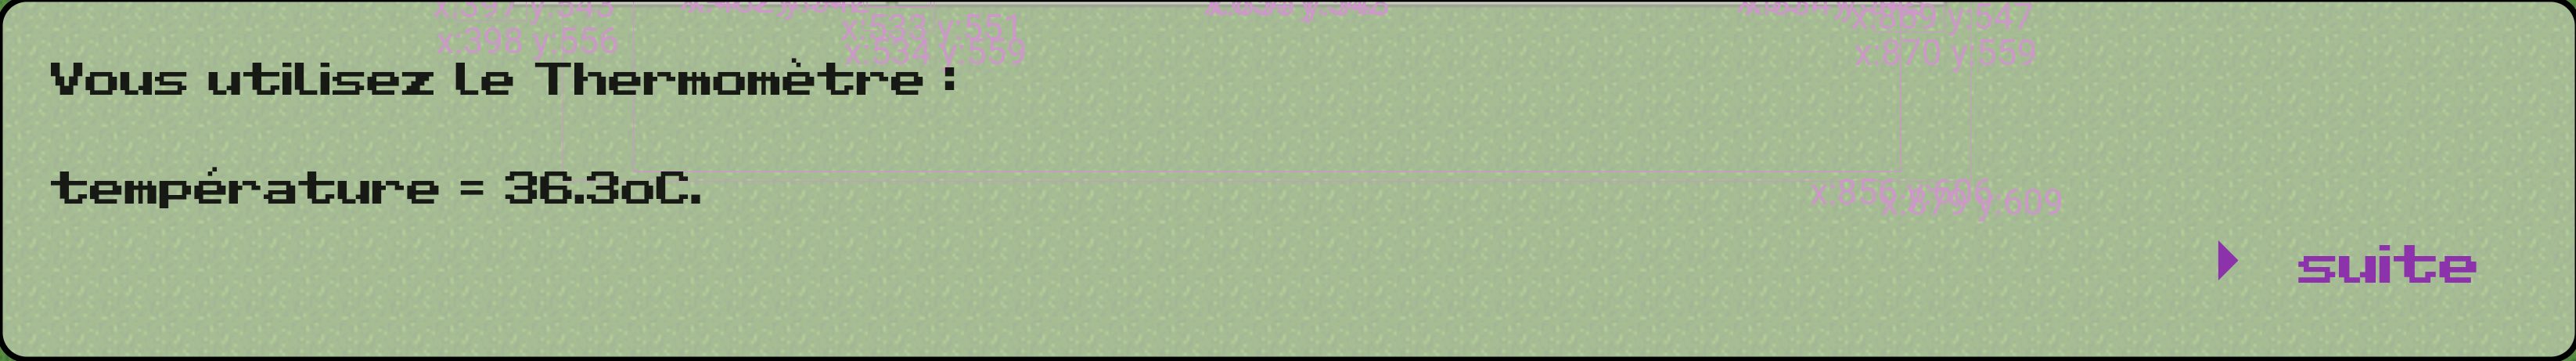
\includegraphics[width=0.8\textwidth ]{images/toolsMenu/toolCanBeUsed.png}
    \caption{Sac à dos - Outils de mesure utilisé}
    \label{fig:pic_dessus}
\end{figure}

%============================================================
%****************Onglet 2 planning*******************

\subsubsection*{Planning de la journée}
\addcontentsline{toc}{subsubsection}{Planning de la journée}

Le second onglet du menu du sac à dos est le planning. En cliquant sur cet onglet, l'utilisateur a la possibilité de visualiser son planning de la journée. \\

\begin{figure}[H]
    \centering
    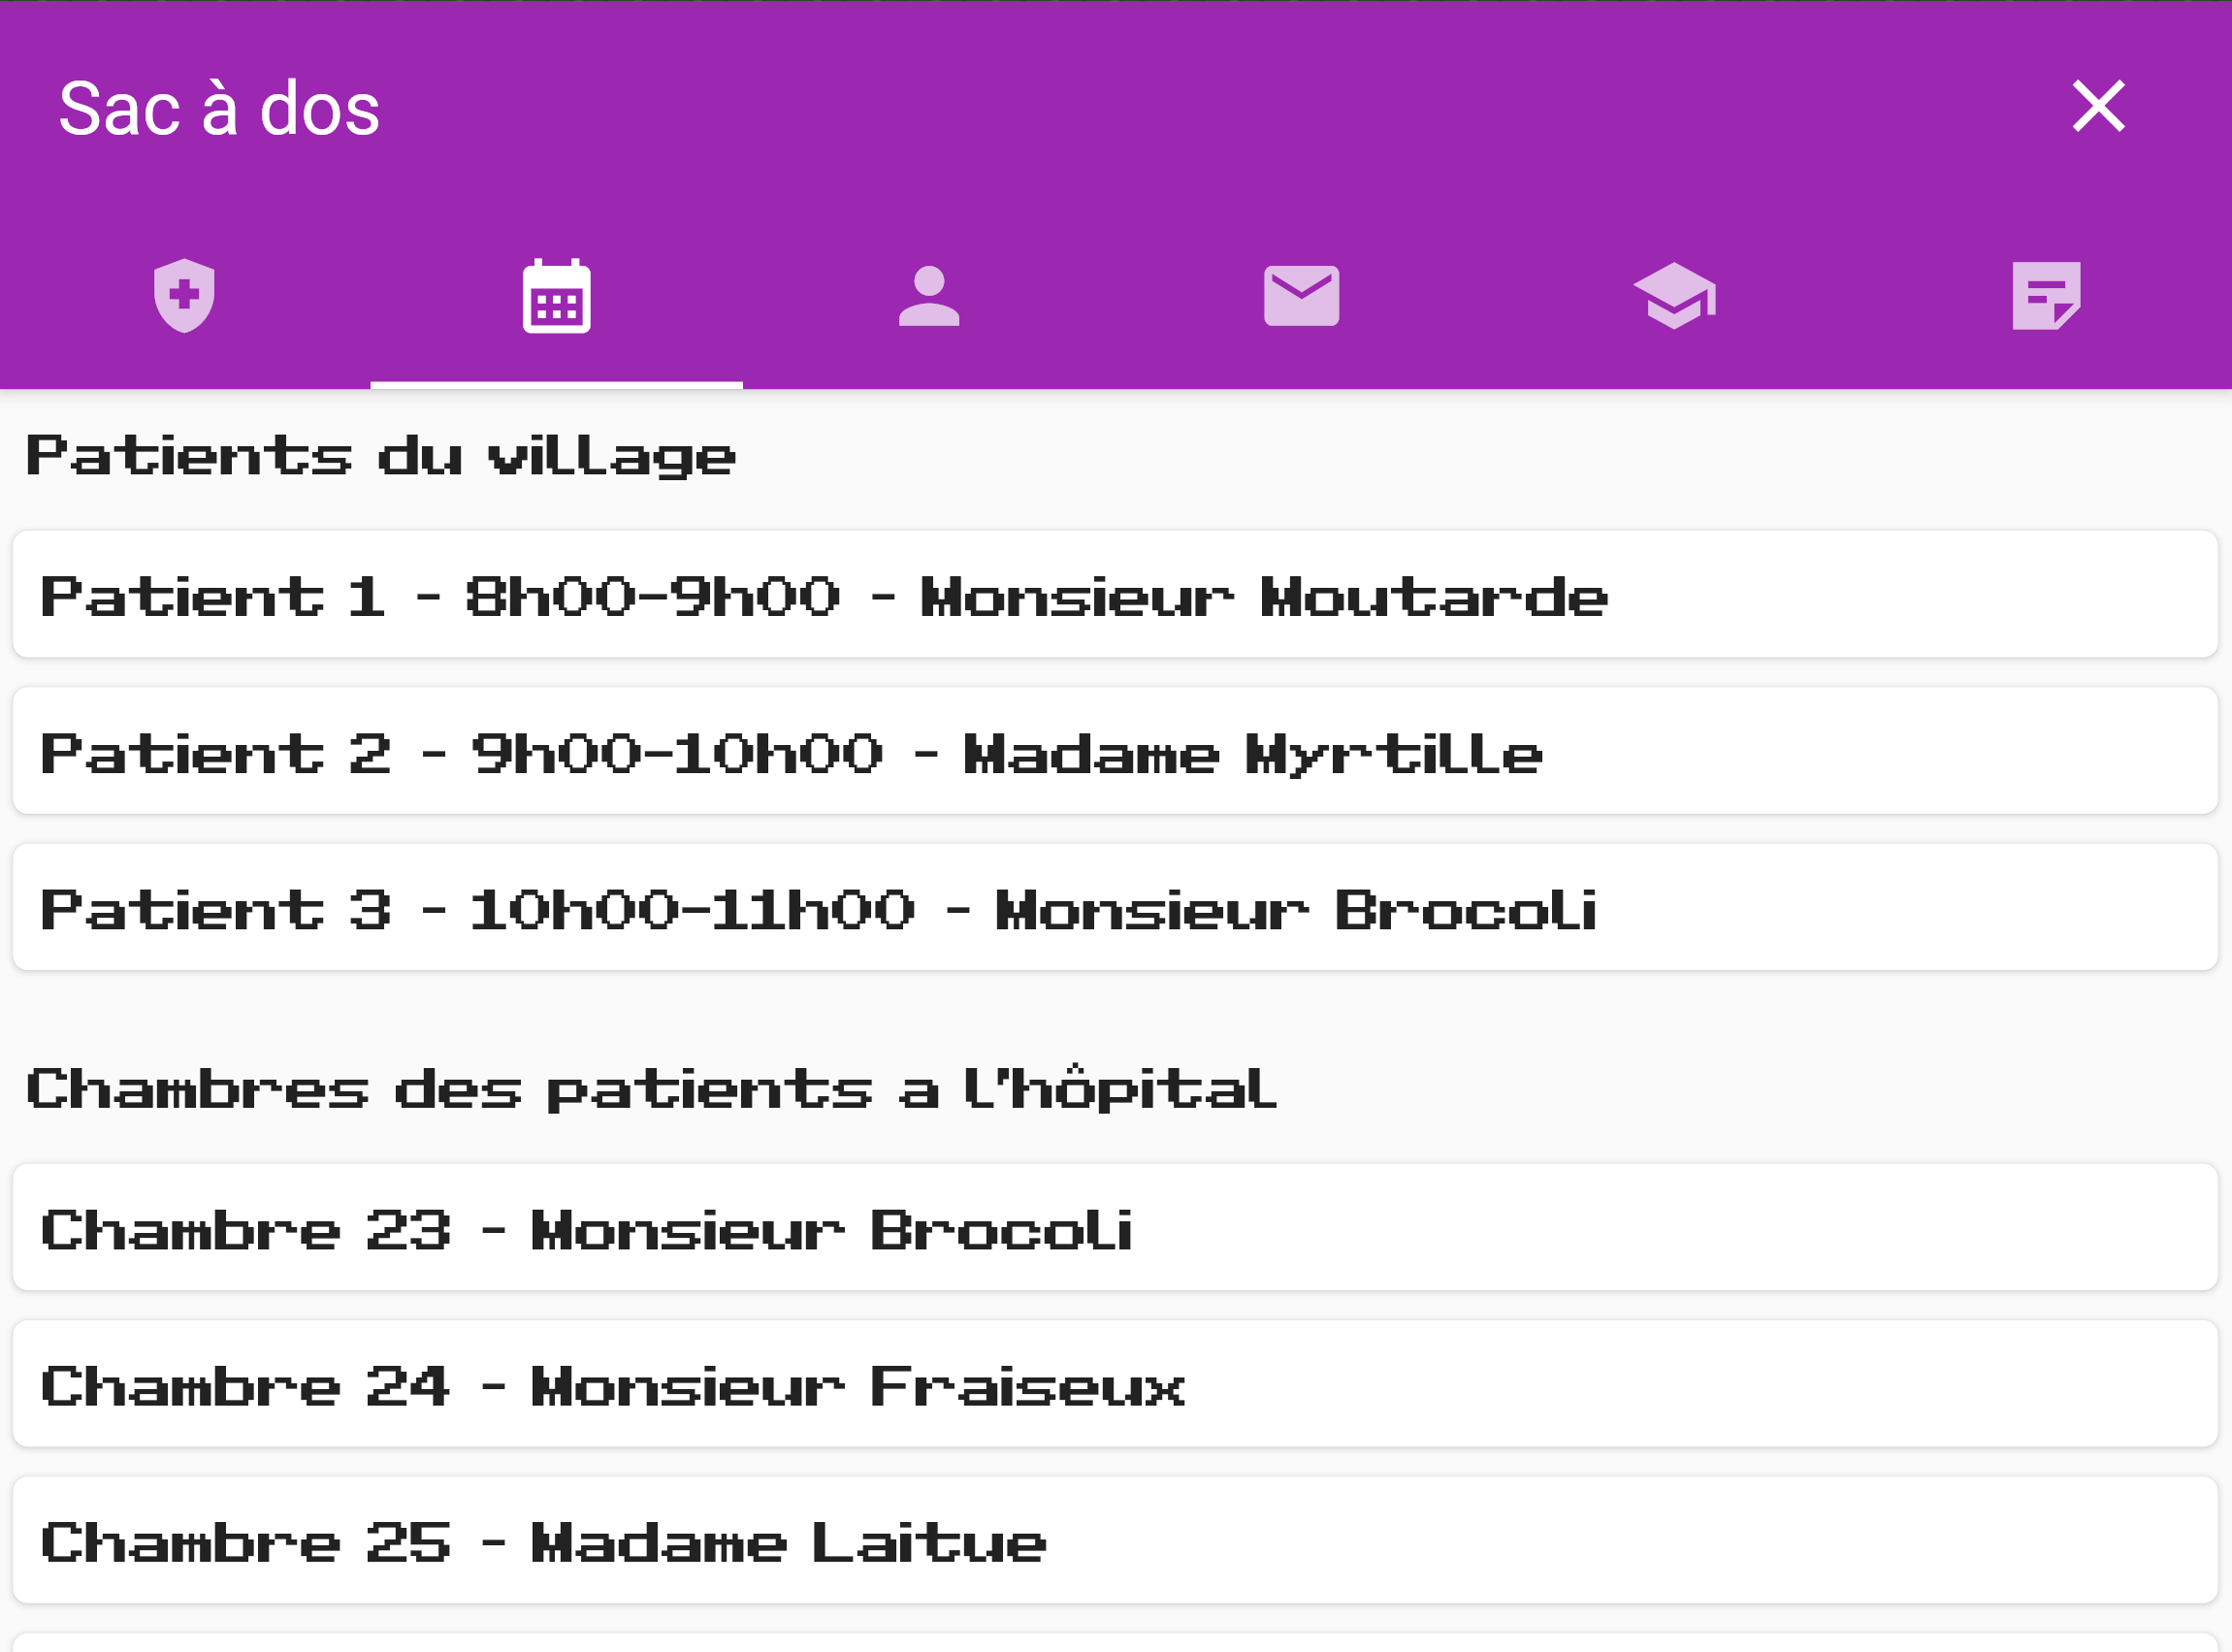
\includegraphics[width=0.8\textwidth ]{images/toolsMenu/planning.png}
    \caption{Sac à dos - Planning de la journée}
    \label{fig:pic_dessus}
\end{figure}

%============================================================
%****************Onglet 3 Situation des patiens*******************

\subsubsection*{Situation des patients}
\addcontentsline{toc}{subsubsection}{Situation des patients}

Le troisième onglet du menu du sac à dos est la situation des patients. En cliquant sur cet onglet, l'utilisateur a la possibilité de visualiser la situation des différents patients à consulter. \\

\begin{figure}[H]
    \centering
    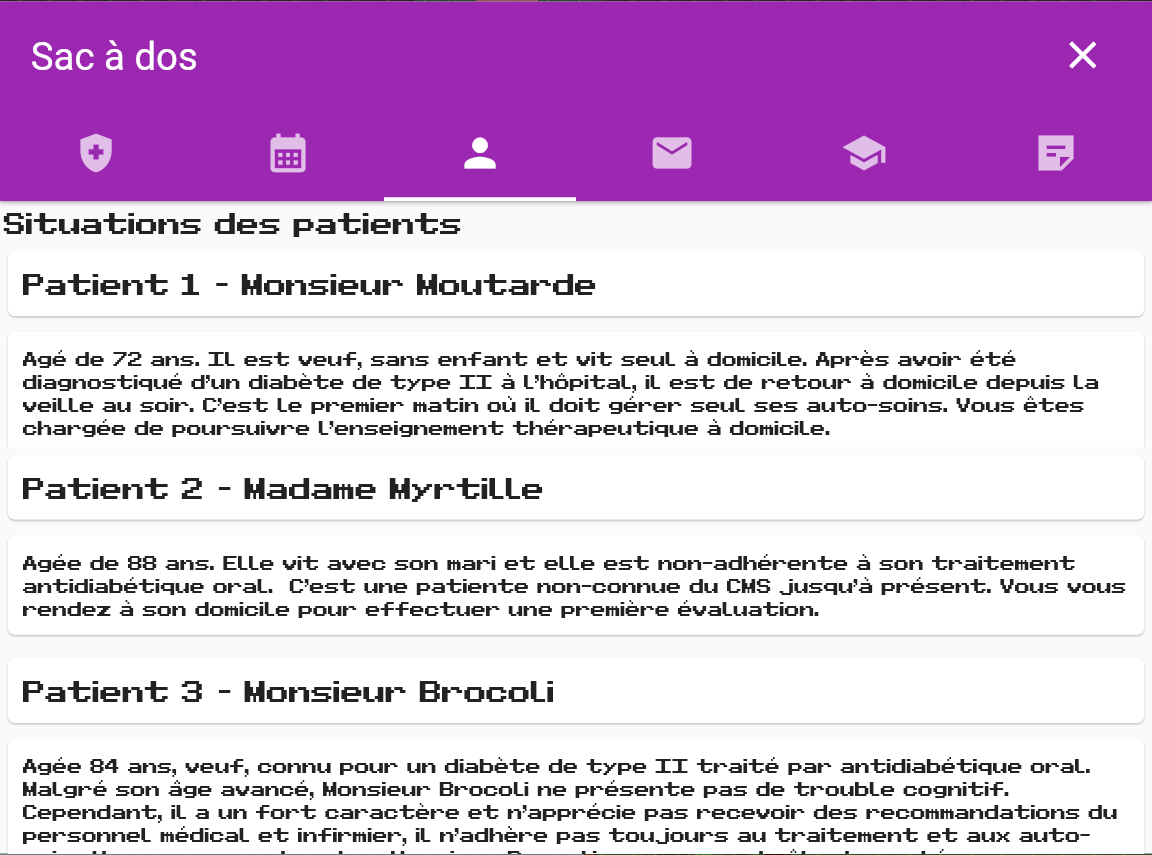
\includegraphics[width=0.8\textwidth ]{images/toolsMenu/situations.png}
    \caption{Sac à dos - Situations des patients}
    \label{fig:pic_dessus}
\end{figure}

%============================================================
%****************Onglet 4 Contacts*******************

\subsubsection*{Contacts}
\addcontentsline{toc}{subsubsection}{Contacts}

Le quatrième onglet du menu du sac à dos contient les contacts. En cliquant sur cet onglet, l'utilisateur a la possibilité de contacter différentes personnes au cours de son jeu. \\

\begin{figure}[H]
    \centering
    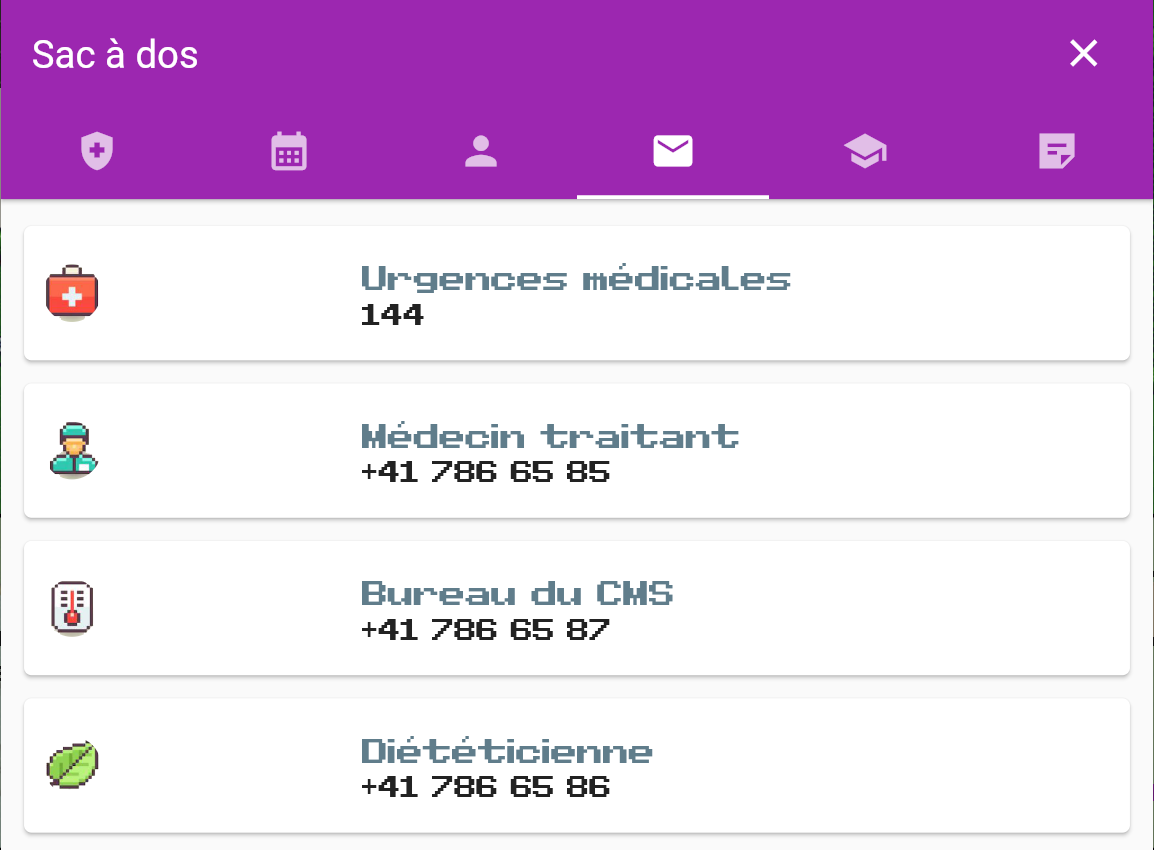
\includegraphics[width=0.8\textwidth ]{images/toolsMenu/contacts.png}
    \caption{Sac à dos - Contacts}
    \label{fig:pic_dessus}
\end{figure}

En cliquant sur un contact alors qu'il n'en a pas l'utilité, un dialogue s'affiche.
\begin{figure}[H]
    \centering
    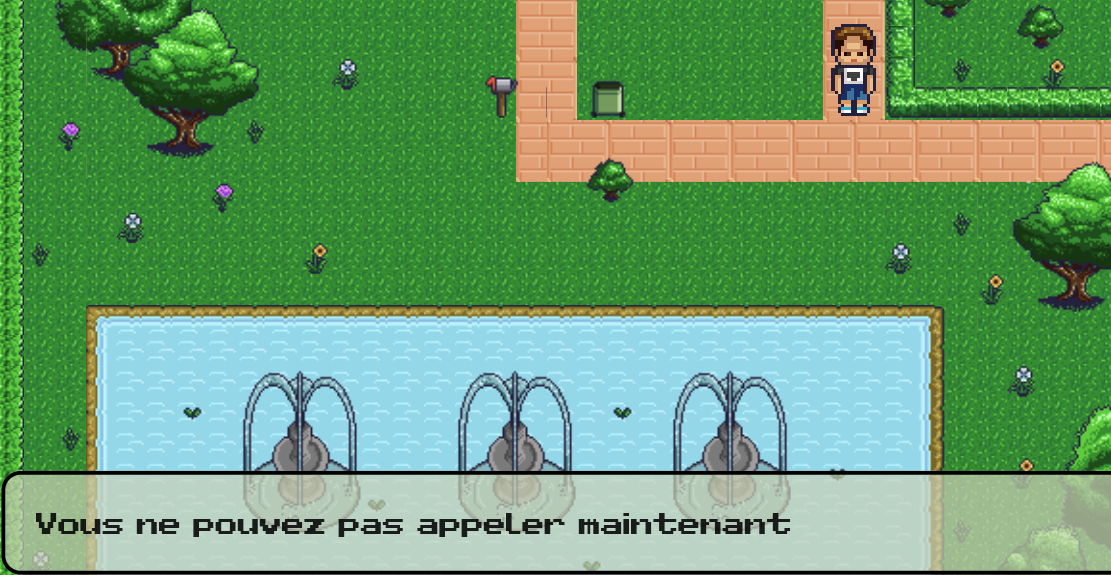
\includegraphics[width=0.8\textwidth ]{images/toolsMenu/contactCantBeUsed.png}
    \caption{Sac à dos - Contact ne peut être appelé}
    \label{fig:pic_dessus}
\end{figure}

En revanche, lorsqu'un contact peut être atteint, un dialogue vous l'indique.
\begin{figure}[H]
    \centering
    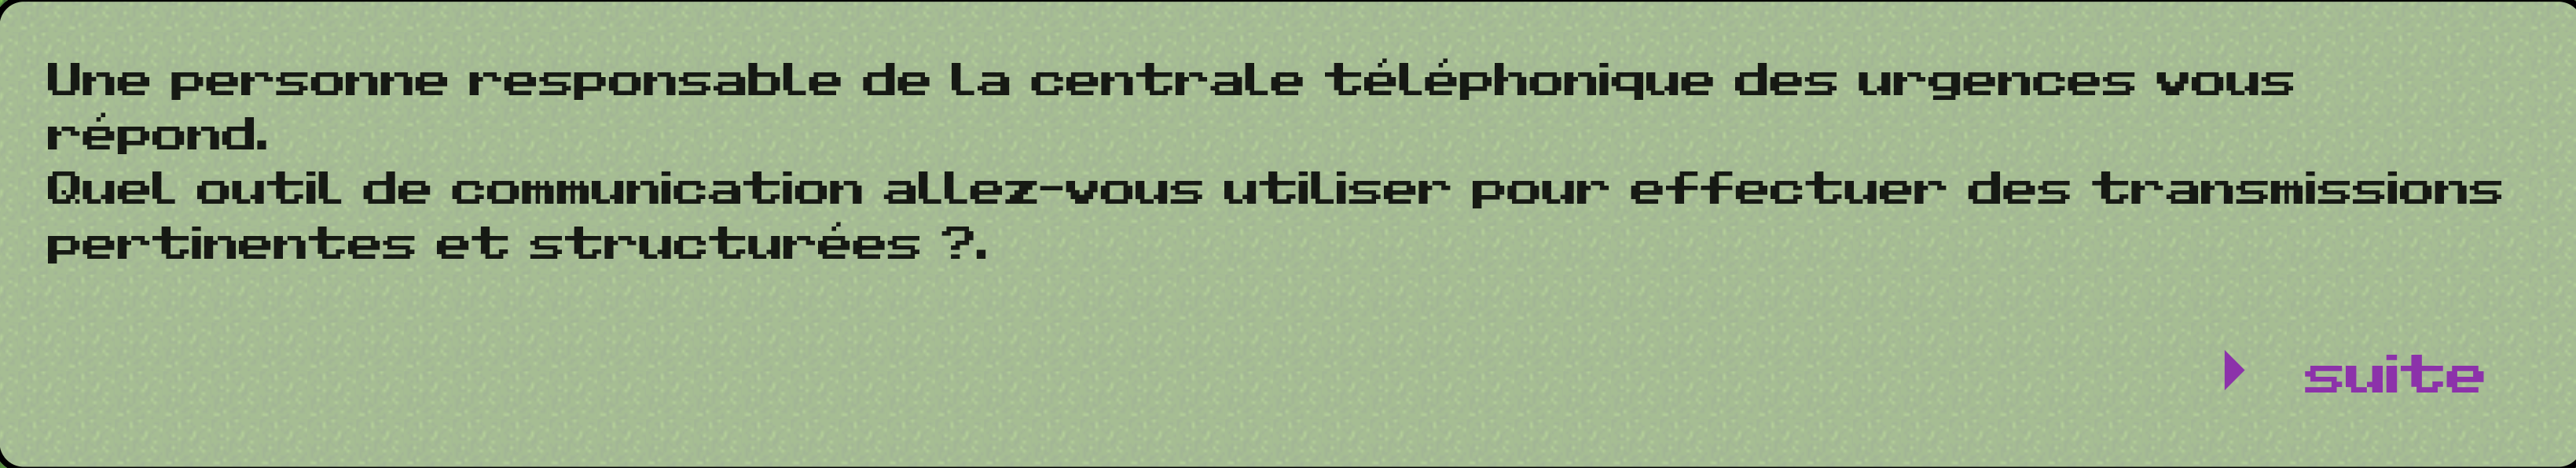
\includegraphics[width=0.8\textwidth ]{images/toolsMenu/contactCanBeUsed.png}
    \caption{Sac à dos - Contact appelé}
    \label{fig:pic_dessus}
\end{figure}

%============================================================
%****************Onglet 5 Collection d'apprentissage*******************

\subsubsection*{Collection d'apprentissage}
\addcontentsline{toc}{subsubsection}{Collection d'apprentissage}

Le cinquième onglet du menu du sac à dos contient les collections d'apprentissage. En cliquant sur cet onglet, l'utilisateur a la possibilité de visualiser les différentes collections d'apprentissage qui lui seront décernées au cours du jeu. \\

\begin{figure}[H]
    \centering
    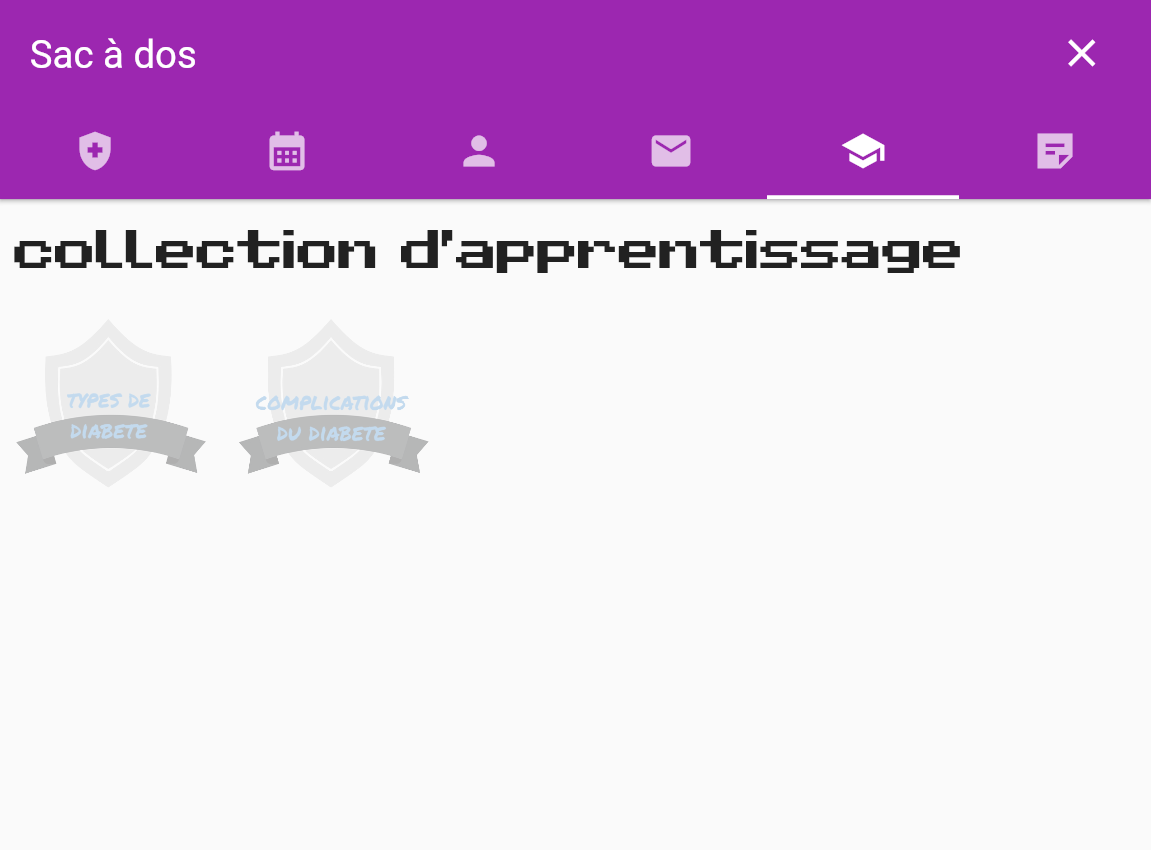
\includegraphics[width=0.8\textwidth ]{images/toolsMenu/collections.png}
    \caption{Sac à dos - Collections}
    \label{fig:pic_dessus}
\end{figure}

%============================================================
%****************Onglet 6 Notes*******************

\subsubsection*{Notes}
\addcontentsline{toc}{subsubsection}{Notes}

Le sixième onglet du menu du sac à dos contient les notes. En cliquant sur cet onglet, l'utilisateur a la possibilité de visualiser les différentes notes des patients qu'il aura visités au cours du jeu. \\

\begin{figure}[H]
    \centering
    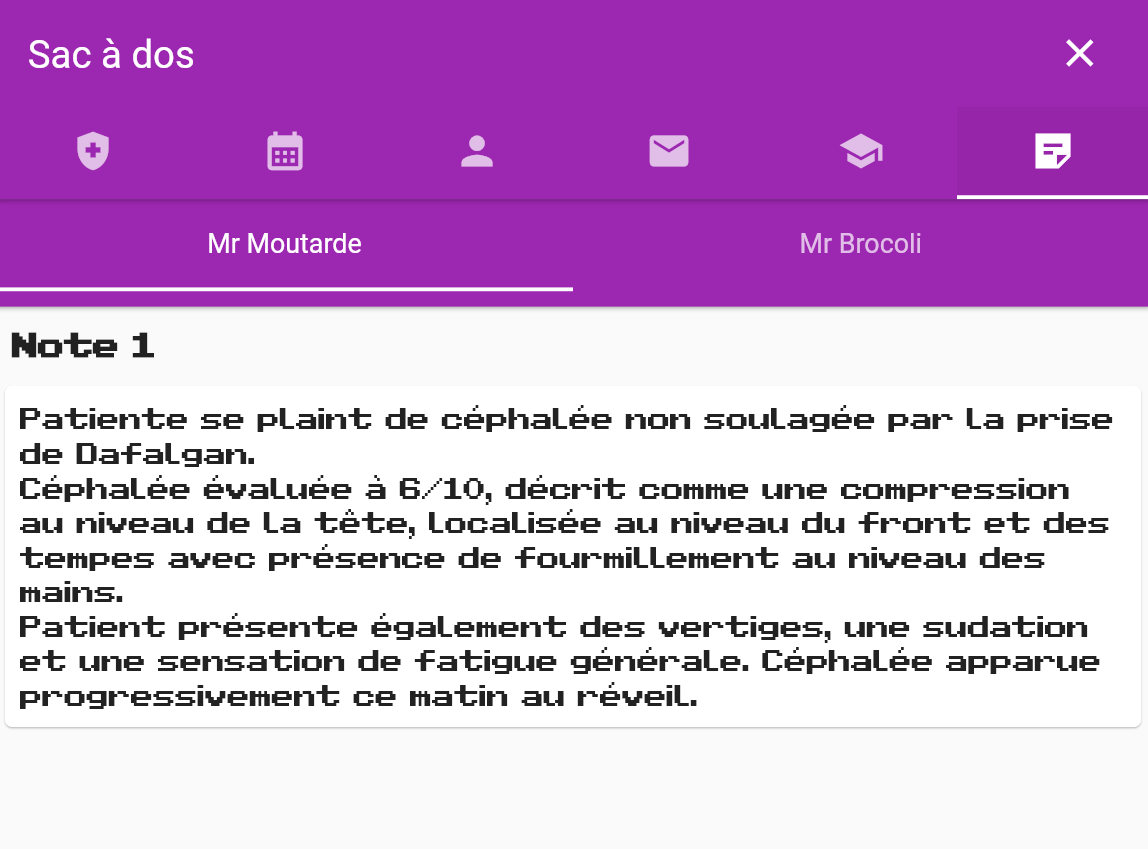
\includegraphics[width=0.8\textwidth ]{images/toolsMenu/notes.png}
    \caption{Sac à dos - Notes}
    \label{fig:pic_dessus}
\end{figure}
